% AAAI-27 AI for Social Impact (AISI) special track submission.
% Two-column AAAI format. Drop the official aaai2027.sty and aaai.bst from the
% AAAI-27 Author Kit next to this file before compiling. Double-blind: authors are
% anonymized. Prose is written without em-dashes, colons, and semicolons by request.
%
% To compile once the Author Kit style is present:
%   pdflatex aaai27_equicharge && pdflatex aaai27_equicharge
% A minimal fallback preamble (for local preview only, NOT for submission) is left
% commented below.

\documentclass[letterpaper]{article}
\usepackage{aaai2027}   % official AAAI-27 style (from the Author Kit)
\usepackage{times}
\usepackage{helvet}
\usepackage{courier}
\usepackage[hyphens]{url}
\usepackage{graphicx}
\usepackage{booktabs}
\usepackage{amsmath,amssymb}
\usepackage{natbib}
\usepackage{caption}
\frenchspacing
\setcounter{secnumdepth}{0}
\setlength{\pdfpagewidth}{8.5in}
\setlength{\pdfpageheight}{11in}

% ---- Fallback preamble for local preview without the Author Kit (commented) ----
% \documentclass[letterpaper,twocolumn,10pt]{article}
% \usepackage[margin=0.75in]{geometry}
% \usepackage{times,graphicx,booktabs,amsmath,amssymb,natbib,caption,url}

\pdfinfo{
/Title (The Price of a Fair Charge)
/Author (Anonymous)
}

\title{The Price of a Fair Charge. Equitable Electric Vehicle Charging Access under
Grid Scarcity, and the Tariff Design that Delivers It}

\author{Anonymous Submission}

\begin{document}
\maketitle

\begin{abstract}
As electric vehicles reach lower income drivers, the fairness of public charging
becomes an access question. A charging site draws power through a fixed grid
connection, so at busy hours it must ration. Operators price by tier, through
memberships, dynamic pricing, and fast versus slow products, and drivers sort into
those tiers by budget in a way that correlates with income, so a revenue maximizing
allocation under scarcity routes the scarce power to the higher margin tiers and
leaves lower income drivers undercharged, a disparate impact rather than deliberate
income discrimination. Using an exact offline solver on a real data calibrated
simulator we characterize this at optimality, verify across several station types that
it is specific to power scarce sites and fades where power is not the binding
constraint, and reach three findings that a utility, operator, or regulator can act on.
First, the price of fairness is paid in the
operator's revenue, not in total service. Equalizing tier satisfaction costs about ten
percent of margin weighted revenue while it raises mean satisfaction and roughly
doubles the worst served tier, although this is a redistribution the premium tier pays
for, since it gives up about eleven points of satisfaction, a consequence of concave
saturating utility that we report rather than sell as free. Second, only an income
neutral tariff removes the disparate impact, cutting the systematic tier gap by about
ninety percent, while a subsidy aimed at the poorest tier alone does not close it and
instead shifts the burden to the middle tier. Third, grid capacity is a second and
independent lever, with a threshold that is metric dependent at about fifty to seventy
kilowatts. We release a fair charging benchmark on the Chargax simulator, with a
corrected two stage oracle, the fairness layer, the baselines, and a state augmented
learning environment. No online controller reaches positive worst decile satisfaction,
far below the oracle ceiling, which defines the open control problem. Our contribution
is the problem formulation, the actionable characterization, and the tariff and grid
levers it exposes. As a second and separate pillar we show that a welfare shaped learned
controller, trained adequately and evaluated on inclusive metrics where a rejected
driver counts as a zero, beats the rule based controllers an operator would deploy. It
earns more profit, serves its drivers more fully, and rejects fewer of them, winning on
each of these on eight or nine of ten seeds and on every measured axis at once on seven
of ten. Control experiments pin the mechanism. The advantage is not that the welfare
reward is merely dense, since two matched magnitude controls that strip its content, a
plain delivered energy signal and a saturating but target blind one, both fail to
reproduce the gain and collapse below the heuristics. What the controller needs is the
demand aware content, a signal of how far each driver is from its own charging target,
which acts as a scheduling prior that completes the drivers who are behind. We are equally
careful about what this is not. The equity weight is not a
tunable between tier fairness dial, which we report as a negative result, and the between
tier disparate impact remains an offline phenomenon that the tariff, not the controller,
addresses.
\end{abstract}

\section{Introduction}

Public charging is becoming everyday infrastructure, and as it does the question of
who it serves well is becoming a question of equity. Electric vehicle ownership is
still skewed toward higher income households, and the drivers who most depend on
public rather than home charging, renters and lower income households, are exactly
the ones for whom charging deserts and high effective prices bite hardest
\citep{sovacool2016,hsu2021,caulfield2022}. At the same time a charging site is a
scarce resource allocator. A single fast charger can request more than one hundred
kilowatts, and a site connection is often rated well below the sum of what its
chargers could pull at once, so when several cars plug in together the operator has
to ration power. Most controllers in this space optimize profit, because it is easy
to measure and it pays the bills, but profit does not care who gets served. Operators
already price by tier, through memberships, dynamic pricing, and fast versus slow
products, and drivers sort into those tiers by budget in a way that correlates with
income. A revenue seeking allocation under scarcity therefore routes the limited
power toward the higher margin tiers and lets the others leave with half empty
batteries. Because tier tracks income, the effect is a disparate impact on lower
income drivers rather than any deliberate income discrimination, which is the version
of the problem a real operator and a real regulator would recognize.

We take that observation as a policy problem rather than only a control problem. If
a station must ration power, who ends up powered, what does it cost to ration
fairly instead, and what lever should a decision maker pull. We answer with an
exact offline solver on a real data calibrated environment, and we lead with the
findings that a utility rate designer, a charging network operator, or a regulator
can use.

\paragraph{The findings, stated for a decision maker.}
The efficiency and equity objectives do conflict once drivers sort into priced tiers,
but the conflict is narrower and more actionable than a naive reading suggests. The
price of fairness is paid in the operator's revenue, not in aggregate service. On our
scarce reference site the profit optimal schedule holds the low margin tier near forty
percent of its requested energy while giving the high margin tier about ninety four
percent, and equalizing the tiers costs about ten percent of margin weighted revenue.
The value we place on the redistribution is a choice we make explicit. Under equal
weighting of a satisfied kilowatt hour across tiers, equalization raises mean
satisfaction from about seventy two to about eighty four percent and lifts the worst
tier from about forty to about eighty three percent, so it is close to free in
aggregate. It is not free to everyone. The premium tier gives up about eleven points
of satisfaction, from about ninety four to about eighty three percent, and the
aggregate gain is positive only because charging satisfaction saturates. A driver
does not want more than a full battery, so the premium tier sits near the flat top of
a concave utility while the budget tier sits on its steep part, and energy moved from
the former to the latter buys more satisfaction than it costs. Our contribution is not
the sign of this effect, which is the classical implication of concave utility, but
its magnitude on a realistic charging model and the decomposition below of how much of
it is priced and how much is physical. The gap is created by the spread of margins
across tiers, and only removing the spread removes it. Equalizing the margins, by an
income neutral tariff, cuts the tier gap by about ninety percent, whereas both natural
partial fixes fail. A subsidy to the lowest tier alone shifts the unmet demand onto the
middle tier, and a cap on the premium tier alone leaves the budget tier still the
lowest paying and still starved. The lever is the spread, not either end. Grid capacity
is a separate lever that removes the scarcity forcing the rationing, and we report the
capacity at which the gap effectively disappears, which turns a demonstration into a
capacity planning target.

\paragraph{Contributions.}
(1) A problem formulation. We cast online EV charging under a grid limit as welfare
optimal control over an endogenous, streaming, and partly policy controlled
population, with a per customer utility that counts rejected and undercharged
drivers rather than only the ones who left happy. (2) An actionable characterization.
Using a corrected clairvoyant oracle we show the price of fairness is a revenue cost
not a service cost, we identify the tariff design that closes the price driven equity
gap and the subsidy that fails to, and we quantify the grid capacity range for the
scarcity driven residual. (3) A learned controller that is useful online. As a second
pillar we show that a welfare shaped policy, trained adequately and judged on inclusive
metrics, beats the rule based controllers an operator would deploy on profit, inclusive
service, within population inequality, and rejection at once, without winning by turning
marginal drivers away. This is an efficiency and service result, and control experiments
isolate it to the demand aware content of the welfare signal, its measure of how far each
driver is from its own target, since neither a plain energy control nor a target blind
saturating one of matched magnitude reproduces it. We pair it with an
explicit negative result, that the equity weight is not a tunable between tier fairness
dial, and the between tier disparate impact stays the tariff's story rather than the
controller's. (4) A
released benchmark and the open problem it surfaces, that no online policy reaches
positive worst decile satisfaction, far below the oracle ceiling, which is the online to
offline gap we invite others to close.

\section{Related work}

\paragraph{Energy justice and mobility equity.}
Our framing draws on the energy justice literature, which organizes fairness in
energy systems into distributional, procedural, and recognition dimensions
\citep{sovacool2016,jenkins2016}. The distributional strand is the one we make
operational, and it connects to the large body of work on energy burden and energy
poverty, where low income households spend several times the income share on energy
that higher income households do \citep{bednar2020,drehobl2020}. In transport
specifically, work on electric vehicle access and charging deserts documents that
public charging availability and price fall unevenly across income and race
\citep{hsu2021,caulfield2022,khan2022}. We use these ideas to motivate the ability
to pay model rather than as decoration, and we tie the segment weights to income
terciles and the energy burden gradient.

\paragraph{Welfare economics and fair division.}
Our objective is a social welfare function over per driver satisfaction. The
inequality aversion is the Atkinson index and its equally distributed equivalent
\citep{atkinson1970}, the worst off limit is the Rawlsian difference principle
\citep{rawls1971}, and the capability view of why access rather than payment is the
right space is due to Sen \citep{sen1999}. The one parameter alpha fair family we
sweep originates in network resource allocation \citep{mo2000} and sits inside the
broader theory of fair division and collective welfare \citep{moulin2003}. Framing
the welfare choice inside this tradition is what makes it a defensible position
rather than an arbitrary pick.

\paragraph{Electricity rate design.}
Because our sharpest policy lever is the tariff, we build on the applied economics
of electricity pricing. The distributional incidence of nonlinear and time varying
pricing is studied by \citet{borenstein2012} and \citet{burger2020}, and the design
of time of use and demand charge tariffs by \citet{faruqui2011}. This literature is
what lets us say which realistic tariff designs move the equity gap and which do not.

\paragraph{Fairness as a learned objective.}
A line of work optimizes a nonlinear concave welfare of a vector of per user returns
inside a Markov decision process. \citet{siddique2020} show that a state augmented
with accrued reward is needed because the objective is not additive, and further
work studies the Nash welfare axiomatically and algorithmically
\citep{mandal2023,fan2023,ju2024}. All of these assume a fixed and known set of
beneficiaries present throughout. Our population is a stream of arrivals and
departures whose membership the policy influences, which is what motivates the
bounded sufficient statistic augmentation.

\paragraph{Online fair division and general utility RL.}
A second line studies online allocation of a divisible resource to agents that
arrive over time under a nonlinear welfare \citep{barman2022,banerjee2022,
sinclair2022}, including a Markov decision process re-solving heuristic that uses
learning only as a baseline \citep{hassanzadeh2023}, and reusable resources with
finite holding times under a time averaged max min \citep{liu2025}. These are
planning or online algorithm methods that assume a forecastable demand model and
mostly no departures. A third line lets the objective be a nonlinear function of the
state occupancy of a single system \citep{zahavy2021,mutti2022}. We need a welfare
across a set of distinct and transient drivers, and the finite trial view of
\citet{mutti2022} is the reason we evaluate the welfare on the realized day.

\paragraph{Fair electric vehicle charging.}
Within the charging literature fairness is usually proportional or max min fairness
handled by convex optimization or model predictive control, or, when reinforcement
learning is used, an after the fact index of equality added to the reward. We
instead make a principled and adjustable social welfare the object of study, we model
heterogeneous ability to pay so the tradeoff is the one real charging equity is
about, and we build on the Chargax simulator \citep{ponse2025}.

\section{Problem setting}

\paragraph{A real data calibrated environment.}
Chargax models a station as a tree of power nodes with a hard limit at the grid
connection. Time advances in five minute steps and one episode spans a single day,
a fixed horizon of 288 steps. At each step the agent picks a discrete charging level
for every charger and for the on site battery. The distributions the environment
samples are empirical rather than synthetic. Arrival times, dwell times, per session
energy demand, and the vehicle fleet come from Chargax's measured datasets, and the
electricity price is the real Netherlands day ahead series for 2021 to 2023. We state
what is real and what is modelled explicitly in the released data documentation, and
we provide an adapter to the public Caltech ACN-Data session dataset
\citep{lee2019acndata} as an independent calibration.

\paragraph{Differentiated pricing, and why this is a disparate impact.}
A real charging operator does not infer a driver's income and ration power by it,
which would be operationally strange and legally fraught. What operators do run is
differentiated pricing, namely membership and subscription tiers, dynamic and
congestion pricing, and product tiers such as fast versus level two, each carrying a
different per kilowatt hour margin. Drivers sort into these tiers by budget, and tier
membership is documented to correlate with income, with lower income drivers
clustering in the lower margin tiers and relying most on public rather than home
charging. We therefore model each segment as a price tier characterized only by the
margin the operator earns from it, drawn independently of battery size. We ground the
tier margins in a real affordability structure rather than pick them for convenience.
Each tier corresponds to a household income tercile, and its margin is its
willingness to pay per kilowatt hour relative to the median under a sub proportional
income elasticity, which yields about 0.6, 1.0, and 1.5 for the budget, mid, and
premium tiers, corroborated by the energy burden gradient. Given tiered margins a
revenue maximizing allocation under scarcity mechanically favors the higher margin
tiers, and because tier correlates with income the effect is that lower income
drivers are systematically under served. This is a disparate impact of revenue
optimal allocation, not deliberate income discrimination by the operator, and it is
the distributional justice concern our oracle makes quantitative. The operator never
observes income, so the analysis does not rest on a contested demographic proxy, and
the policy levers we study act on the pricing structure and the grid, not on any
inference of who a driver is. We are explicit that the direction of the disparate
impact, that the lower income tier is the one under served, follows by construction
from the mapping of income to a lower margin tier, so it is a modeling assumption
grounded in the energy burden and charging access literature
\citep{drehobl2020,hsu2021,khan2022} rather than an independent empirical finding of
this paper. What the analysis contributes is not the direction but the magnitude of
the gap, the spread mechanism that produces it, and the pricing and capacity levers
that remove it, none of which is implied by the mapping alone.

\paragraph{Per driver utility.}
For a driver $i$ we define satisfaction as the fraction of requested energy delivered
by the time the driver leaves,
\begin{equation}
u_i = \mathrm{clip}\!\left(\frac{\text{delivered}_i}{\text{desired}_i},\,0,\,1\right),
\end{equation}
with desired energy equal to the energy needed to reach the requested level at
arrival. We evaluate $u_i$ for every driver in the realized stream, not only for the
ones who left satisfied. A driver who hits the deadline half charged keeps that low
score, a driver still plugged in at the end of the day is counted by flushing the
station at the horizon, and a rejected driver receives a zero. Counting the rejected
and the undercharged is what stops a policy from looking fair by serving only the
easy cases or by turning the needy away, and it is well posed only because admission
and departure are treated as endogenous.

\paragraph{Welfare objective.}
Group the drivers into segments $g$ and write $u_i$ for the satisfaction of driver
$i$. We optimize the equally distributed equivalent form of the alpha fair welfare,
\begin{equation}
W \,=\, \Psi_g\Big(\big\{\,\mathrm{EDE}_\alpha(\bar\phi_g)\,\big\}\Big),
\qquad
\bar\phi_g = \frac{1}{N_g}\sum_{i \in g}\phi_\alpha(u_i),
\end{equation}
where $\phi_\alpha$ is the isoelastic kernel, $\mathrm{EDE}_\alpha$ is its inverse,
and $\Psi_g$ is either the population weighted pool, which recovers individual alpha
fairness, or a soft minimum across segments, which is an egalitarian stance
\citep{atkinson1970,mo2000,rawls1971}. With $\alpha$ equal to zero this is mean
satisfaction, with $\alpha$ equal to one it is the geometric mean, and as $\alpha$
grows it leans toward the worst off. The reward blends profit and welfare through an
equity weight $\lambda$ in the unit interval,
\begin{equation}
r_t = (1-\lambda)\,\frac{\Delta \text{profit}_t}{\text{scale}} \,+\, \lambda\,\big(W_{t+1}-W_t\big).
\end{equation}
The normalization constant scale is the approximate daily profit of a profit blind
max charge policy on the reference site, about two hundred euros per day, so that the
episode profit return and the bounded welfare return are on a common footing and a
given $\lambda$ denotes the same efficiency and equity mix across configurations.

\paragraph{Why the formulation is the contribution.}
Two properties make this more than standard fair reinforcement learning. The set of
beneficiaries is not fixed, and a charge sensitive car departs once satisfied, so the
policy moves the very population it is scored on. And the welfare is a nonlinear
function of the whole realized distribution, so it is not a sum of per step rewards.
We view welfare optimal control over an endogenous, policy influenced beneficiary
population, with departure realized non additive utility, as a formulation the
community has not cleanly posed, and the machinery below is what makes it tractable.

\section{Method}

\paragraph{A bounded sufficient statistic.}
Each welfare we use is a generalized mean, so it depends on the drivers only through
a small fixed size summary. For segment $g$ we keep a count $N_g$ and a kernel sum
$S_g$ equal to the running total of $\phi_\alpha(u_i)$ over drivers that have left or
been rejected. The pair $(N_g,S_g)$ is a sufficient statistic for the welfare
regardless of how many drivers stream through, so the state stays small. We append a
normalized version of it, the present unmet demand per segment, and the fraction of
the day elapsed, to the observation. This is the streaming analogue of the accrued
reward state used for a fixed set of objectives in earlier work \citep{siddique2020}.

\paragraph{Welfare as an exact undiscounted return, densely shaped.}
Defining the per step reward as the change in welfare and summing over the fixed
horizon without discounting telescopes to $W_T - W_0$, and since $W_0$ is constant
the undiscounted return is exactly the welfare of the final allocation. The identity
holds only at a discount of one, which is why we optimize the undiscounted daily
return. Because satisfaction is realized only at departure this signal is sparse, so
we define a potential $\Phi(s)$ equal to the welfare that would be realized if every
connected car departed now at its current satisfaction, on top of the drivers that
already left or were rejected. Using $\Phi(s_{t+1})-\Phi(s_t)$ is potential based
shaping in the sense of \citet{ng1999}, so it leaves the optimized objective equal to
the final welfare while firing on most steps rather than only at departures. A
rejected driver enters the welfare as a zero, which requires drawing the attributes
of each arriving driver before deciding whether a charger is free, a sample then
reject modification of the simulator. We optimize with proximal policy optimization
\citep{schulman2017} at a discount of one on the state augmented environment.

\paragraph{A corrected offline oracle.}
To separate the difficulty of the problem from the difficulty of learning we solve a
clairvoyant linear program over per driver per step energy, subject to the grid power
limit, a per car power cap, and a per car energy demand. It can maximize total
satisfaction, value weighted delivered energy, or the worst off segment. The maximin
variant matters for soundness. A single epigraph program that maximizes the worst off
value returns an allocation that levels the better off down to that value, which
reports a perfectly equalized outcome below what is provably achievable. We instead
solve two stages. The first maximizes the worst off segment mean, and the second
holds that value fixed and maximizes total delivered satisfaction, so the returned
allocation is Pareto efficient and its worst segment can never fall below what the
profit optimum already delivers. We report the true two stage maximin and, for
transparency, the strict equalization outcome that levels down.

\section{Results}

The numbers below come from the released run and match the released results table
exactly. The offline findings use sixteen realized days on the scarce reference site,
sixteen charger connectors behind a thirty kilowatt grid, with the grounded price
tiers. We define two quantities we report throughout. A tier's satisfaction is its
mean over drivers and days. The tier gap is the difference between the best and the
worst tier on that day-averaged satisfaction, so it measures whether a tier is
systematically under served, which is the disparate impact we care about, and it is
by construction exactly the maximum minus the minimum of the per tier column in Table
\ref{taboracle}. It is smaller than the average of each day's own worst to best gap,
because which tier is unlucky on a given day varies, and that day to day variation is
noise rather than a disparate impact. A per day audit over thirty two days confirms
this reading is not a definitional trick. Under the value weighted tariff the same tier,
the budget tier, is the worst served on thirty one of the thirty two days, so the gap is
systematic and the day averaged and per day measures agree, both near five tenths. Under
an income neutral tariff the worst served tier instead roams across the three tiers,
roughly a third of days each, so no tier is systematically starved and the day averaged
measure collapses to near four hundredths while the per day gaps remain as noise. The
averaged measure and the per day measure coincide exactly when the impact is systematic
and diverge exactly when it is noise, which is the behaviour a disparate impact measure
should have.

\paragraph{The price of fairness is a revenue cost, not a service cost.}
Table \ref{taboracle} and Figure \ref{figoracle} report the clairvoyant solver. The
profit optimal allocation gives the mid and premium tiers most of what they ask for
and holds the budget tier near forty percent, a tier gap of about 0.54, and at this
scarce reference site the budget tier is the one starved on thirty one of thirty two days,
though this systematic starvation is specific to power scarce sites, as we show below. The
corrected two stage maximin equalizes the three tiers at about 0.83 while delivering the
same total energy as the profit optimum. That last point is exact rather than average.
On every one of the thirty two days the profit, utilitarian, and maximin optima deliver
the identical total energy, to within solver tolerance, because the grid is the binding
constraint, so the objectives only redistribute a fixed quantity and never change how
much is served. Moving from the profit optimum to the maximin optimum therefore costs
margin weighted revenue, a median of about nine percent and a per day range of two to
eighteen, while mean satisfaction rises from about 0.72 to about 0.84 and the worst tier
rises from about 0.40 to about 0.83. As discussed above this aggregate gain is a consequence of
saturating utility and comes with a real loss to the premium tier, so the tension is
between the operator's revenue and the distribution, not between total service and
equity. The corrected maximin also removes an artifact of a naive single stage
program, which levels every tier down to about 0.36 and misstates the price of
fairness as a large cut in mean satisfaction.

\begin{table}[t]
\centering
\caption{Offline oracle on the scarce site with three ability to pay segments.
Entries are mean satisfaction per segment, with the operator's value weighted revenue
in the last column. The profit optimum starves the budget segment for revenue. The
true segment maximin equalizes without leveling down and delivers the same energy, so
equity costs revenue, not service. Strict equalization is shown to expose the leveling
that a naive maximin would report.}
\label{taboracle}
\begin{tabular}{lccccc}
\toprule
tier objective & budget & mid & premium & gap & revenue \\
\midrule
profit optimal        & 0.40 & 0.84 & 0.94 & 0.54 & 402 \\
utilitarian           & 0.89 & 0.84 & 0.82 & 0.08 & 356 \\
tier maximin (true)   & 0.84 & 0.84 & 0.83 & 0.01 & 364 \\
strict equalization   & 0.82 & 0.82 & 0.82 & 0.00 & 358 \\
\bottomrule
\end{tabular}
\end{table}

\begin{figure*}[t]
\centering
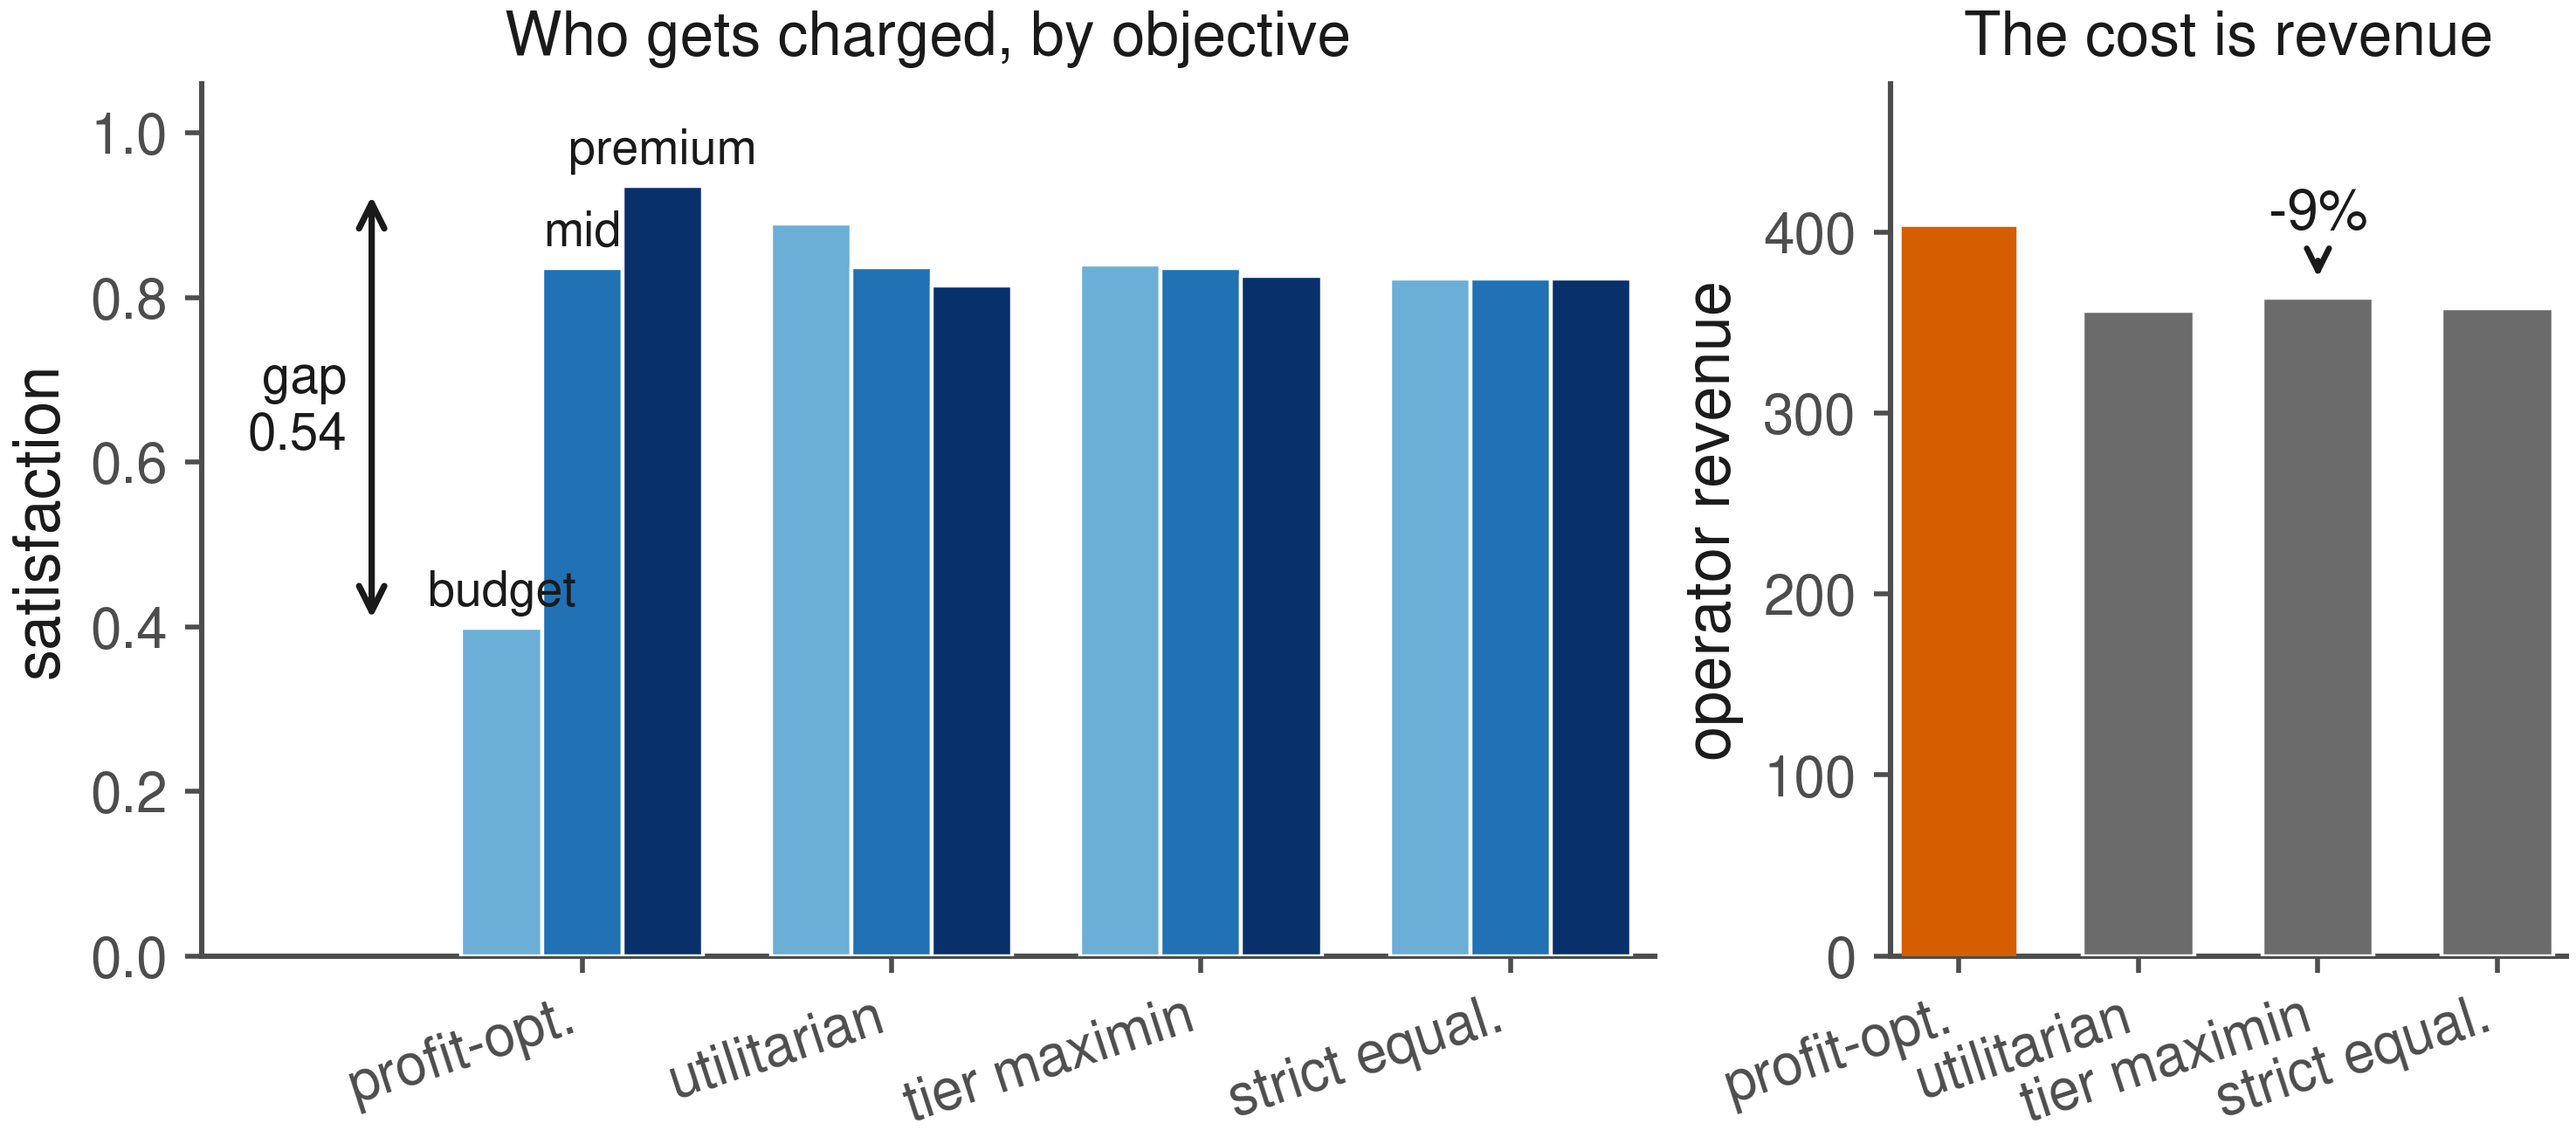
\includegraphics[width=0.86\textwidth]{figures/oracle_tradeoff.png}
\caption{Left, per segment satisfaction under each clairvoyant objective. The profit
optimum starves the budget segment while the equity objectives equalize near the
utilitarian level. Right, the operator's revenue. The price of fairness is paid here,
not in aggregate satisfaction.}
\label{figoracle}
\end{figure*}

\paragraph{The aggregate gain is a redistribution premium drivers pay for.}
We stress that the mean satisfaction rise under equalization is not a free lunch. It
is the classical consequence of concave saturating utility, and it comes with a real
loss to the premium tier, which drops from about 0.94 to about 0.83, roughly eleven
points, while the budget tier gains about forty four points. To check that this is not
an artifact of one price gradient we swept the premium tier margin from 1.2 to 3.0. The
premium loss stays near eleven points and the budget gain near forty four points
throughout, and the revenue price of fairness grows with the gradient from about eight
to about fourteen percent. The finding we claim is therefore the magnitude on a
realistic charging model and the decomposition into a priced and a physical part, not
the sign, and the free in aggregate reading holds only if a satisfied kilowatt hour is
weighted equally across tiers, which is a value choice we state rather than hide.

\paragraph{The disparate impact is a function of the margin spread, and only removing
the spread closes it.}
This is our central and most actionable finding, and Table \ref{tabtariff} and Figure \ref{figtariff} are the
evidence. Under the status quo tiered tariff the profit optimal tier gap is about 0.54
and the systematically under served tier is the budget tier. The natural partial
interventions both fail, and they fail for the same reason. A subsidy to the lowest
tier alone does not close the gap. The best any budget only credit reaches is about
0.28, and once the budget margin reaches parity the budget tier is no longer uniquely
worst off, but the burden does not vanish, it lands on whichever of the budget and
middle tiers the profit maximizer now finds cheapest, mid on nineteen of thirty two
audited days and budget on the other twelve, so the gap persists. Symmetrically, a cap
on the premium tier alone does not close it either. Capping the premium margin down to
the middle level, or even below it, leaves the gap near 0.50 with the budget tier worst
served on thirty one of thirty two days, because the budget tier is still the lowest
paying and so still the first the profit maximizer starves. Neither end helps on its own, because
what drives the disparate impact is the spread of margins across tiers, not the level
of any one of them. The gap closes, to about 0.04, only when the margins are made
equal, whether by an income neutral flat tariff or by compressing every tier to a
common level. The residual 0.04 is not tier correlated, so it is day to day noise
rather than a disparate impact. The policy rule is therefore sharp. Reducing the
spread is what removes the disparate impact, and a credit for the poorest tier or a cap
on the richest, applied alone, does not. Temporal designs such as time of use or demand
charges are tier agnostic and do not touch the spread at all. Grid capacity, described
next, is a separate lever that removes the scarcity rather than the spread.

\begin{table}[t]
\centering
\caption{Rate design and the tier gap. Both partial interventions fail. A subsidy to
the poorest tier alone shifts the burden to the middle tier, and a cap on the premium
tier alone leaves the budget tier starved. Only equalizing the margins, by an income
neutral tariff or by full compression, removes the gap. The disparate impact is a
function of the margin spread.}
\label{tabtariff}
\begin{tabular}{lccc}
\toprule
tariff design & margins & tier gap & worst tier \\
\midrule
tiered (status quo)          & 0.6, 1.0, 1.5 & 0.54 & budget \\
budget subsidy to parity     & 1.0, 1.0, 1.5 & 0.28 & mid/budget \\
budget subsidy past parity   & 1.8, 1.0, 1.5 & 0.54 & mid \\
premium cap to middle        & 0.6, 1.0, 1.0 & 0.50 & budget \\
premium cap below middle     & 0.6, 0.8, 0.8 & 0.51 & budget \\
income neutral (equal)       & all equal     & 0.04 & none \\
\bottomrule
\end{tabular}
\end{table}

\begin{figure}[t]
\centering
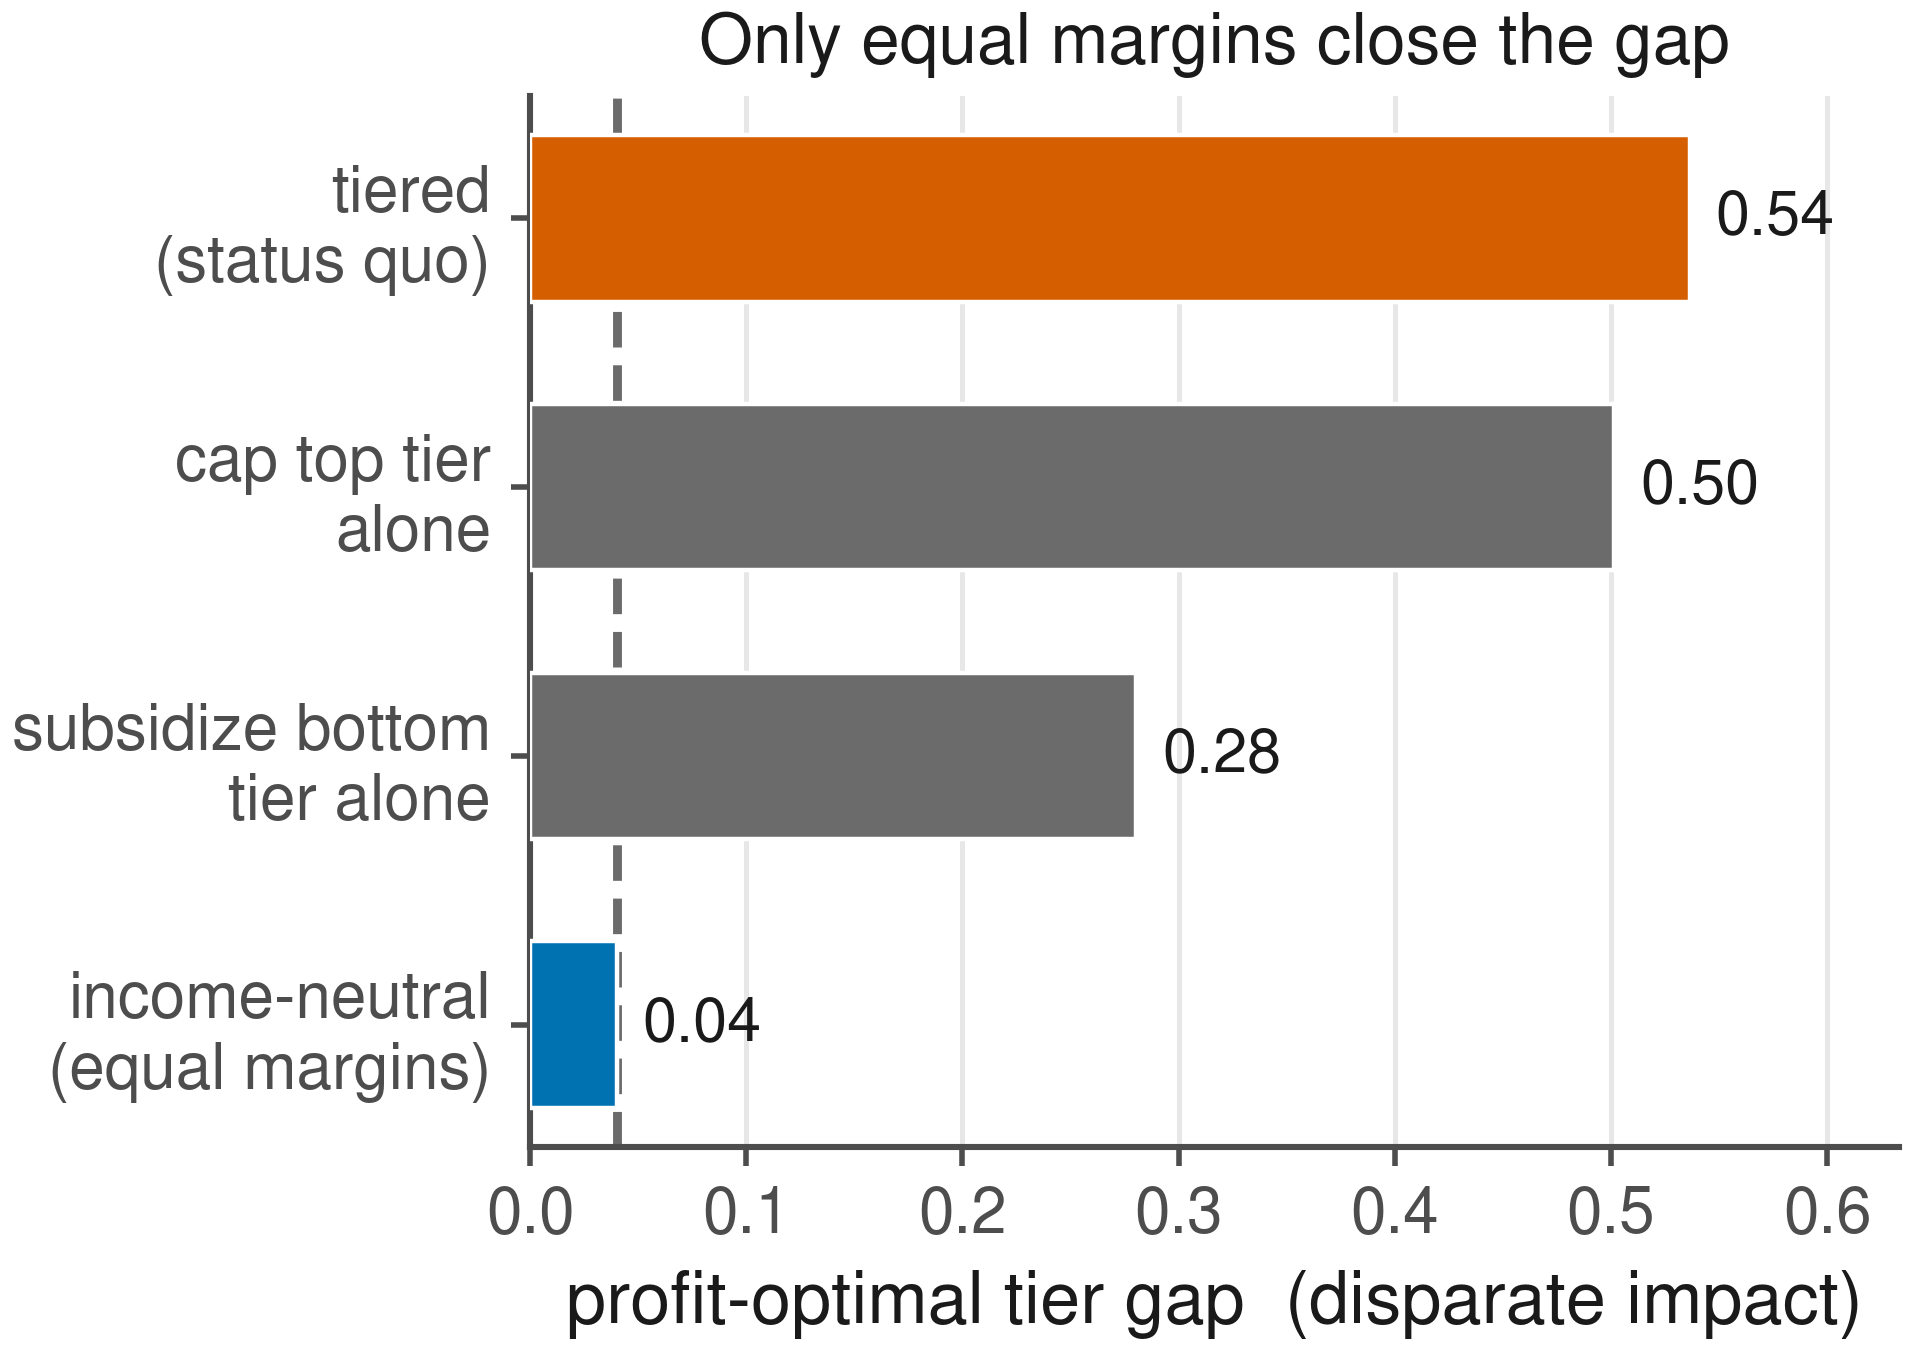
\includegraphics[width=0.82\linewidth]{figures/rate_design.png}
\caption{The disparate impact is a function of the margin spread. Both partial
interventions fail, capping the top tier alone and subsidizing the bottom tier alone,
and only an income neutral tariff with equal margins reaches the scarcity floor (dashed).}
\label{figtariff}
\end{figure}

\paragraph{Grid capacity is the second, independent lever.}
Figure \ref{figcapacity} sweeps the grid connection under the profit blind max charge
policy and under the clairvoyant profit optimum. Enough capacity removes the scarcity
that forces rationing at all, and both the Gini and the tier gap fall steeply and then
flatten. We report this as a range rather than a sharp threshold, because the oracle
tier gap is noisy and slightly non monotonic near its floor of about two to three
hundredths above seventy kilowatts, so a single kilowatt value would over claim. By the
Gini of satisfaction the inequality reaches within ten percent of its abundant floor by
about fifty kilowatts, and by the stricter oracle tier gap the disparity is small, below
about five hundredths, from about seventy kilowatts upward. For this sixteen charger
site the disparity is largely gone by roughly fifty to seventy kilowatts, and a planner
reading the stricter metric should size to the upper end. Capacity and pricing address
different causes. Capacity removes the scarcity, and income neutral pricing removes the
spread that decides who loses, so either lever reduces the disparate impact and using
both removes it.

\begin{figure}[t]
\centering
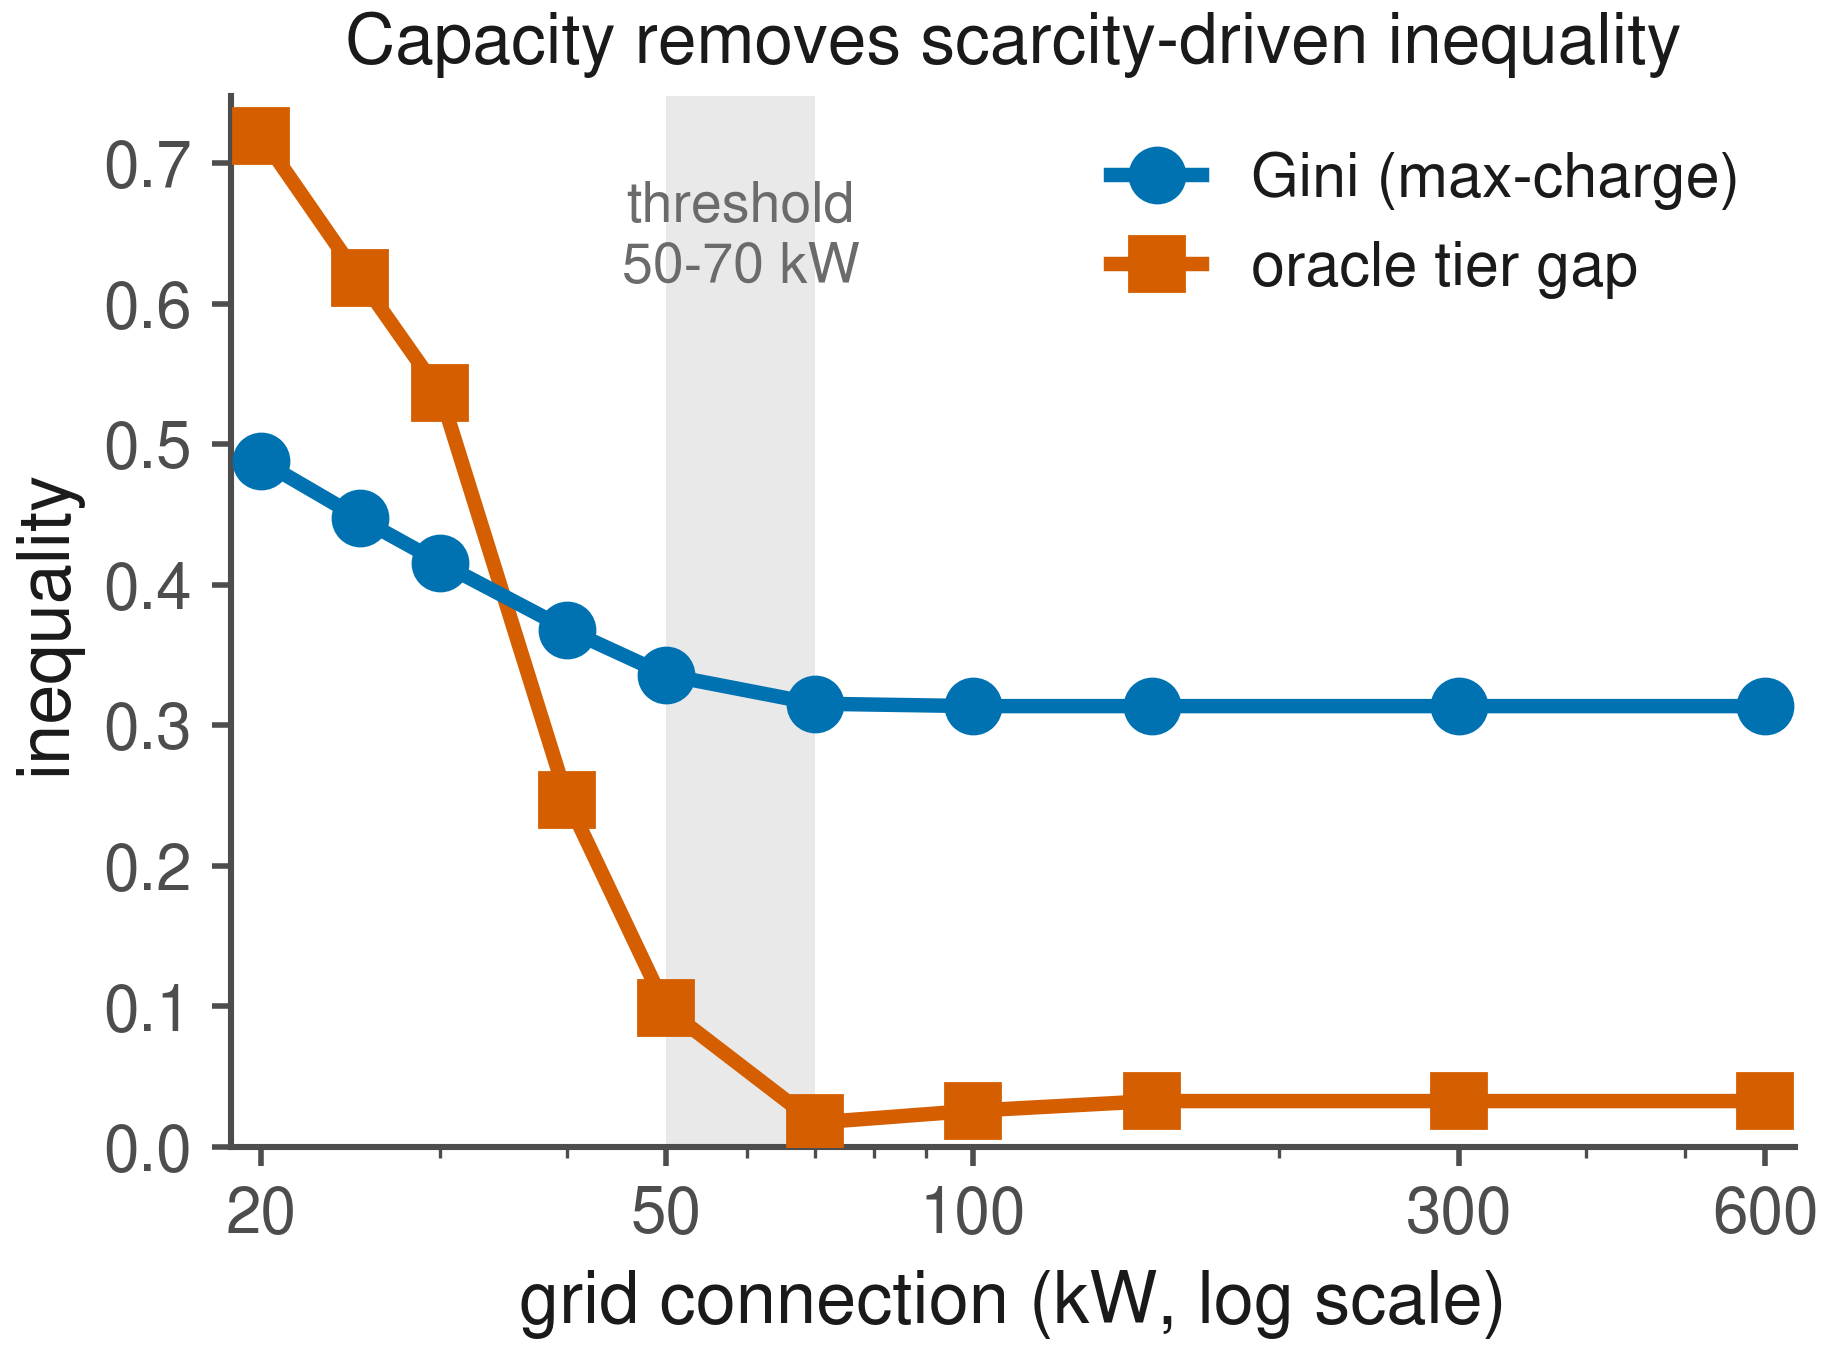
\includegraphics[width=\linewidth]{figures/capacity_threshold.png}
\caption{Inequality against grid capacity. The Gini of satisfaction under max charge
and the clairvoyant profit optimal tier gap both fall toward an abundant floor. The
threshold is metric dependent, about fifty kilowatts by Gini and about seventy by the
oracle tier gap, for this sixteen charger site.}
\label{figcapacity}
\end{figure}

\paragraph{Scarcity is what creates the inequality.}
Consistent with the sweep, the same profit blind policy is markedly more unequal when
power is scarce. On the thirty kilowatt grid its satisfaction Gini is about 0.42 with
mean satisfaction about 0.71, and on an abundant six hundred kilowatt grid the Gini
falls to about 0.31 with mean satisfaction about 0.87. The inequality is a property of
the binding constraint, not of any particular controller.

\paragraph{The disparate impact is a property of power scarce sites, not of tiered
pricing in general.}
Our headline result is established on one site, so we test whether it holds elsewhere by
rerunning the oracle audit at three genuinely different stations (Figure \ref{figrobust}), varying charger count,
grid size, arrival rate, dwell profile, and vehicle fleet. It does not hold everywhere,
and the way it fails is informative rather than damaging. At the scarce residential
reference the budget tier is the worst served on thirty one of thirty two days with a
tier gap near 0.56 and a revenue price of fairness near nine percent. At a high traffic
highway site, also power bound, it persists, budget worst on about four days in five with
a gap near 0.27 and a revenue price of fairness near six percent. But at a workplace site
with long spread dwells and at a low traffic shopping site, power is not the binding
constraint, the profit optimum can serve every tier without rationing, and the disparate
impact largely disappears, with tier gaps below 0.19 and a revenue price of fairness of
essentially zero. The pattern is exactly what the mechanism predicts. The disadvantage
appears when and only when rationing by tier is profitable, which requires power to bind,
so the revenue price of fairness tracks the disparate impact across sites. The claim we
support is therefore the scoped one, that value weighted allocation systematically
disadvantages lower income drivers at power scarce charging sites, which is where the
policy question actually lives, rather than the unqualified claim that tiered pricing
does so everywhere.

\begin{figure}[t]
\centering
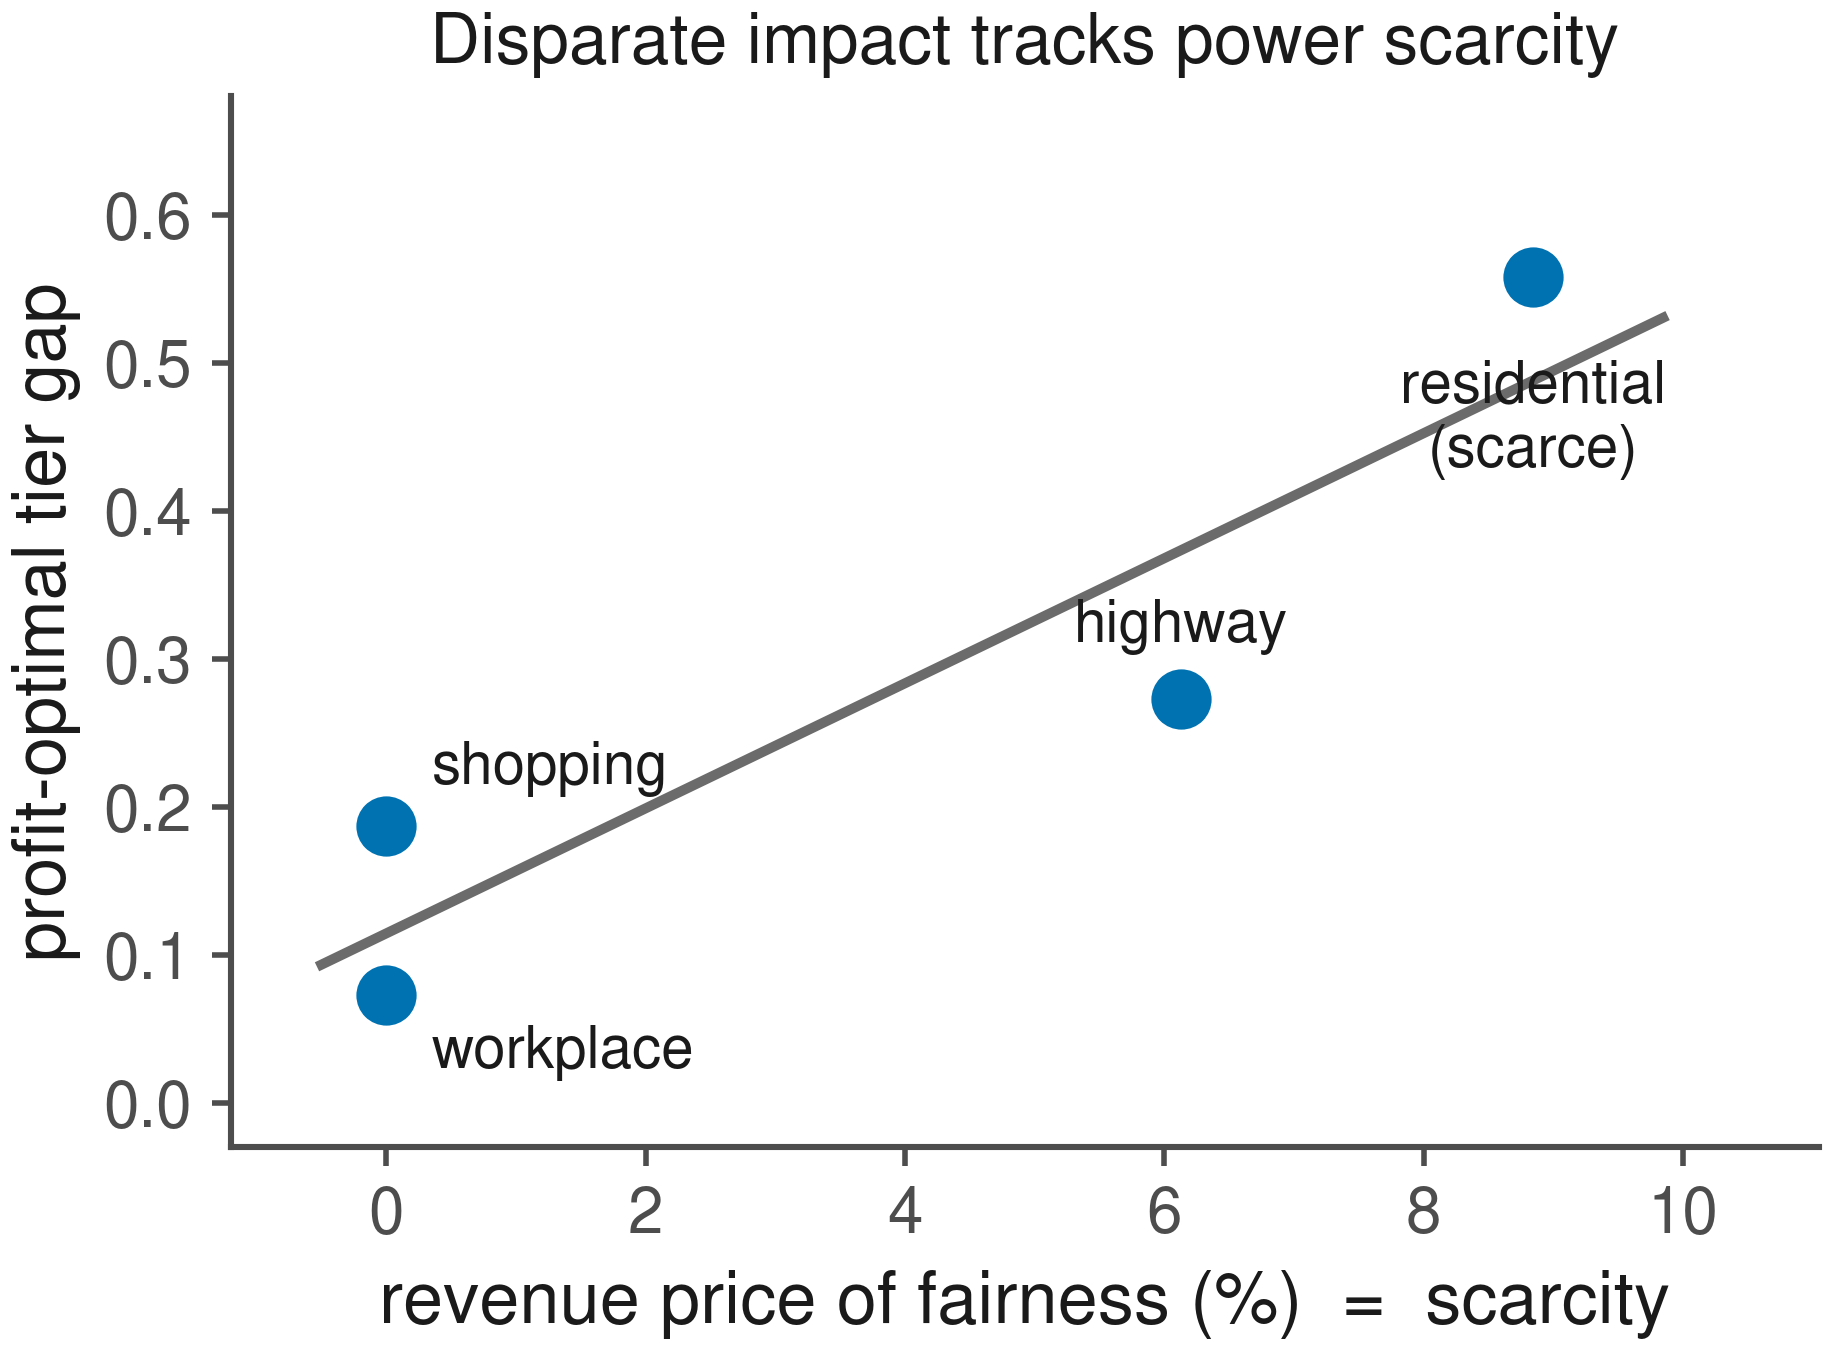
\includegraphics[width=0.82\linewidth]{figures/robustness_sites.png}
\caption{The disparate impact is specific to power scarce sites. Across four station
types, the profit optimal tier gap rises with the revenue price of fairness, which is
positive only when power binds. Where power is not the binding constraint, workplace and
shopping, the gap and the revenue price of fairness are both near zero.}
\label{figrobust}
\end{figure}

\paragraph{Online baselines and the online to offline gap.}
Table \ref{tabrl} places the non learned online baselines against the oracle ceiling.
No online policy achieves positive worst decile satisfaction, far below the ceiling,
so the online to offline gap is the open control problem the released benchmark
defines.

\paragraph{Second pillar. A learned controller beats the heuristics an operator would
deploy, on efficiency and service.}
The offline analysis above is the paper's headline and stands on its own. As a second
and separate contribution we ask whether a learned controller is useful online, and the
answer is yes, on efficiency and service rather than on between tier equity. We train
the welfare shaped policy at an equity weight of one half, for three million steps with
an annealed entropy bonus, over ten seeds, and compare it against the non learned
heuristics on the paper's own inclusive metrics, where a rejected driver counts as a
zero. Table \ref{tabcheck} reports the head to head. Against the strongest heuristic,
max charge, the learned controller wins at the median on all four of profit, inclusive
satisfaction, the within population Gini, and rejection rate, earning about two hundred
euros per day against one hundred eighty six, raising inclusive satisfaction from 0.54
to 0.60 and inclusive welfare from 0.50 to 0.55, lowering the Gini from 0.42 to 0.38,
and rejecting fewer drivers. Stated as win rates over the ten seeds, it beats max charge
on profit in eight, on inclusive satisfaction in eight, on inclusive welfare in eight,
on the Gini in seven, and on rejection in nine, and it dominates on all four axes at
once in seven of the ten. We report the fractions rather than say it dominates, because
three seeds do not. The comparison is against the heuristics, not against our own profit
only run, because a learned profit baseline shares the training budget and dynamics and
would confound the claim.

We check the one failure mode that would make this an artifact. Because served
satisfaction is measured over admitted drivers, a policy could look good by shedding
marginal ones, which the paper's inclusive utility is designed to catch. It does not
happen here, and it fails to happen in the direction that closes the objection rather
than merely surviving it. The learned controller rejects fewer drivers than max charge,
a median rejection of 0.21 against 0.23, an improvement on nine of ten seeds, while
scoring higher on the inclusive welfare that counts the rejected at zero. A policy
cannot be inflating service by turning drivers away when it is both admitting more of
them and scoring higher on the inclusive measure. We state what the other three seeds do,
so the seven of ten is not something a reader has to go and reconstruct. Two of the three
underperform on profit and service while rejecting no more than the baseline, and the
weakest of these, at inclusive welfare 0.46 against 0.50, simply did not learn to charge
fully. The third rejects marginally more than the baseline, 0.238 against 0.232, which is
within seed noise. In none of the three is the shortfall driven by shedding drivers, so
the downside case is weaker service, not metric gaming.

The honest reading is that a welfare shaped learned controller realizes much of the
oracle's efficient and high service region online and beats the rule based controllers
an operator would otherwise run. What the controller does is admit more cars and charge
them more fully, which lifts the whole satisfaction distribution and lowers the within
population Gini. We are careful with the Gini, because it is a fairness coded number. Its
improvement is not tier equalizing redistribution, since between tier disparity is
unchanged, so it is a within population effect rather than a between tier one. The
ablations below show the Gini gain requires the demand aware content of the welfare
signal and is not delivered by a content free potential of matched magnitude, whether
monotone or saturating. We also note that the Gini is computed over the served population
and the learned policy serves more drivers, so the comparison is not over a fixed
population, a caveat we state rather than gloss.

\paragraph{The gain needs the demand aware content of the welfare signal, isolated by
three conditions.}
A natural worry is that the welfare term is merely a dense auxiliary reward that helps
optimization regardless of what it encodes, in which case any dense potential of the same
magnitude would do. We test this with two controls, each at the same intermediate weight
and matched magnitude, that strip the welfare signal in two different ways. The first is a
monotone potential, cumulative delivered energy, which removes both the saturating shape
and the satisfaction content. It fails, falling to about one hundred sixty four euros of
profit and inclusive satisfaction of about 0.51, below max charge, so a dense reward alone
is not enough. This control removed two things at once, so on its own it cannot say whether
the saturating shape or the satisfaction content is responsible. The second control
separates them. It is a saturating but content free potential, per connector delivered
energy against a constant reference clipped to the unit interval, which keeps the
saturating shape but removes the demand information, since it no longer knows how far each
driver is from its own target. If the saturating shape were doing the work, this control
would recover the gain. It does not. It lands at about one hundred sixty five euros and
inclusive satisfaction of about 0.52, indistinguishable from the monotone control and still
below max charge. So the saturating shape is not sufficient. What the controller needs is
the demand aware content, the satisfaction signal that measures delivered energy against
each driver's own target, which lets it complete the drivers that are behind on their own
demand rather than the ones that have simply received little energy. That is a demand aware
scheduling prior, and it is why the welfare shaped controller beats both the pure profit
learner and the rule based heuristics on efficiency and service, and why it lifts the
bottom of the within population satisfaction distribution. This is a within population and
scheduling effect, not a between tier one. The driver a demand aware potential prioritizes
is whoever is behind on its own demand, as likely a premium driver as a budget one, so the
signal does not track ability to pay and the between tier gap does not move. The operative
content is this demand awareness rather than the tier structure of the welfare, which is
consistent with the between tier gap not responding to the weight at all.

\paragraph{The equity weight is not a between tier fairness dial, stated as a finding.}
We also looked for a tunable between tier fairness dial, a policy whose equity weight
moves the between tier gap along a frontier, and we did not find one. Across the weight
we detect no systematic effect on between tier disparity. It stays within seed noise, one
to six hundredths, it is not ordered by the weight, and the tier that ends up worst
served is not even consistently the same one across seeds. The strongest policy sits at
the interior weight of one half rather than at an endpoint, while the pure welfare weight
of one is worse and highly variable, so the pure objective also needs the profit term as
a stabilizing anchor. The welfare shaped signal improves within population service and
scheduling, as above, but it does not give an operator a knob for the between tier
disparate impact. We report this as a negative result rather than hide it, because a
reader who runs the weight sweep will see it, and it keeps the two equity notions apart.
The controller does not reduce the between tier disparate impact, because online that
disparity has not formed.
The disparate impact is large only in the offline profit optimal that rations hard, so it
is the tariff's story told offline, while the controller's story is efficiency and service
told online.

% ---- BASELINE TABLE (auto-generated from results.json) ----
% Auto-generated by experiments/make_paper_tables.py -- do not edit by hand.
\begin{table}[t]
\centering
\caption{Non-learned online baselines on the scarce site, against the clairvoyant oracle ceiling. No online policy reaches positive worst decile satisfaction, far below the oracle. This online to offline gap is the open problem the released benchmark defines.}
\label{tabrl}
\begin{tabular}{lcccc}
\toprule
policy & profit & mean sat & Gini & worst 10\% \\
\midrule
max charge & 186 & 0.71 & 0.42 & 0.00 \\
least laxity & 176 & 0.70 & 0.43 & 0.00 \\
proportional fair & 177 & 0.61 & 0.47 & 0.00 \\
saffe & 175 & 0.60 & 0.48 & 0.00 \\
random & 161 & 0.68 & 0.44 & 0.00 \\
\midrule
oracle ceiling (maximin) & -- & 0.83 & -- & 0.83 \\
\bottomrule
\end{tabular}
\end{table}


% ---- CHECK TABLE, the surviving RL result on inclusive axes (from check.json) ----
% Auto-generated by experiments/make_paper_tables.py -- do not edit.
\begin{table}[t]
\centering
\caption{A welfare-shaped learned controller ($\lambda{=}0.5$, 3M steps, median over 10 seeds) against the non-learned heuristics, on the paper's INCLUSIVE metrics (rejected drivers count as zero). The learned controller beats the strongest heuristic (max charge) on every axis, and rejects \emph{fewer} drivers, so the service win is not survivorship. Win rate is the fraction of 10 seeds beating max charge on that axis.}
\label{tabcheck}
\begin{tabular}{lccc}
\toprule
metric & learned ($\lambda{=}0.5$) & max charge & win rate \\
\midrule
profit (EUR/day) & 200 & 186 & 8/10 \\
inclusive satisfaction & 0.595 & 0.544 & 8/10 \\
Gini (inclusive) & 0.382 & 0.416 & 7/10 \\
rejection rate & 0.213 & 0.232 & 9/10 \\
inclusive welfare & 0.551 & 0.499 & 8/10 \\
\midrule
\multicolumn{4}{l}{dominate all four axes at once: 7/10 seeds} \\
\bottomrule
\end{tabular}
\end{table}


\paragraph{The utility design closes the reject to look fair loophole.}
Because admission is a control decision, a policy could try to look fair by shedding
drivers it would serve poorly. Defining utility over the true arrival stream, with
rejected drivers at zero, closes this. Ablating rejection counting lets the same
policy inflate its apparent welfare by about 0.15 on the reference site, which is the
concrete payoff of modelling the population as endogenous rather than fixed. This is
the property that makes the loophole unavailable to a welfare maximizer.

\section{Path to practice}

\paragraph{The recommendation.} Our central and actionable recommendation is that public
charging under scarcity should be priced on an income neutral basis, or more precisely on
a compressed spread of per kilowatt hour margins across customer tiers, because that is
the single intervention that removes the systematic disadvantage to lower income drivers.
On the reference site it cuts the profit optimal tier gap by about ninety percent, from
about 0.54 to about 0.04, at a cost of about ten percent of the operator's margin weighted
revenue and no loss of total energy served, so the cost is a private revenue transfer, not
a reduction in service, which bounds the size of any credit a regulator would need to fund
it. The two intuitive partial measures both fail and should not be relied on. A subsidy to
the poorest tier alone relocates the shortfall to the middle tier, and a cap on the
premium tier alone leaves the poorest tier still the worst served, because what drives the
disadvantage is the spread of margins, not the level of any one tier. A regulator that
cannot mandate a flat tariff can require the margin spread to be compressed, which is the
general form of the same lever. Where pricing cannot be changed, sizing the grid
connection above the scarcity range, roughly fifty to seventy kilowatts for a site of this
scale, removes the rationing that produces the disadvantage in the first place. These are
two independent levers, and either one materially reduces the disparate impact. Because the
disadvantage is specific to power scarce sites, a regulator does not need a blanket mandate,
the pricing rule can be targeted at the sites where power binds, which our audit identifies
by a positive revenue price of fairness, making the intervention both cheaper and better
aimed.

The route from this work to impact does not require deploying a controller, because
the actionable objects are the tariff and the connection, not the policy. The decision
makers are charging network operators, distribution utilities and their regulators,
and public charging site planners. The decisions the characterization informs are rate
design, equity conditions in charging procurement or regulation, and grid connection
sizing. A regulator concerned that revenue maximizing operators under serve low income
drivers can read from the oracle that requiring equal tier satisfaction costs the
operator about ten percent of margin weighted revenue while raising aggregate
satisfaction, so the bill is a private revenue transfer rather than a loss of total
service, which bounds the size of any needed incentive or credit. A utility rate
designer can read that an income neutral or fully equalizing tariff removes the price
driven gap while a credit for the poorest tier alone does not, which is a concrete
design rule. A site planner can read the capacity threshold, about fifty to seventy
kilowatts depending on the metric, as the connection size beyond which scarcity no
longer drives the disparity. There is also a deployment pathway that does require the
controller. An operator already running a rule based scheduler can replace it with the
welfare shaped learned policy and expect more revenue, higher inclusive service, lower
within population inequality, and fewer rejections at once, which is a concrete online
efficiency and service improvement over the status quo heuristics rather than an adoption
of an analysis. It does not change the between tier disparate impact, which the tariff
addresses. The released benchmark and oracle
let any of these actors re-run the analysis on their own arrival data through the
provided calibration hooks, so the pathway is adoption of the analysis, not of a black
box.

\section{Discussion and limitations}

The result we trust most is the oracle, because it is exact and independent of
optimization, and the correction to its maximin materially changes the headline from a
large service cost to a modest revenue cost that the premium tier pays. The learned
controller is the second pillar and we scope it carefully. Its win over the heuristics
is real, holds on inclusive metrics, and is not survivorship, but it rests on ten seeds
and a single site, and the strongest per seed advantages vary across metrics, so we
state it as a robust ten seed result rather than a guarantee. The equity weight is not a
fairness dial, which we report as a negative result rather than omit. The study has further limits. We disable vehicle to
grid discharging in the main runs to keep the action space small. The oracle relaxes
the nonlinear charge curve and the battery round trip, so it is a valid but loose upper
bound. Segment membership of rejected drivers is attributed by the arrival mix once we
group. The willingness to pay multipliers are grounded in income and energy burden data
but remain a model of demand rather than a measured demand curve, and a real operator's
own segmentation would refine them. The impact axis is the one simulation alone cannot
fully close, which is why the path to practice above is framed around levers a decision
maker already controls.

\section{Conclusion}

We framed EV charging under a grid limit as fair sequential allocation over a stream of
drivers whose membership the controller helps shape, and we used an exact solver on a
real data calibrated environment to reach findings a decision maker can act on. The
price of fairness is a revenue cost and not a service cost, the disparate impact is a
function of the margin spread so that only equalizing the tiers removes it while a
subsidy to the poorest tier or a cap on the richest does not, and a modest increase in
grid capacity removes the scarcity driven residual. As a second pillar we showed that a
welfare shaped learned controller beats the heuristics an operator would deploy on
inclusive service, profit, within population inequality, and rejection at once, an
efficiency and service result, while being honest that its equity weight is not a tunable
between tier fairness dial and that the between tier disparate impact stays the tariff's
story. We release the corrected oracle,
the fairness layer, and the benchmark, and we name the online to offline control gap as
the open problem that follow up work can target.

\section*{Reproducibility statement}

The fairness layer, the baselines, the two stage offline solver, the tariff and
capacity analyses, and the experiment scripts are released with the paper, along with
documentation stating which distributions are real and which are modelled. The
environment is Chargax \citep{ponse2025}. One command runs the reinforcement learning
free core, which produces every offline finding above, and a second runs the full
study including the multi seed learning benchmark. The figures and the results table
are regenerated from the saved run, and the site layout, the arrival regime, the
grounded segment weights, the reward normalization constant, the discount of one, and
the optimizer settings are fixed in the experiment configuration.

\appendix
\section{Appendix. Learned controller, supporting detail}

The body reports the headline learned result, the ten seed inclusive comparison in
Table \ref{tabcheck}. This appendix records two supporting details, the training budget
needed to reach it and the evidence behind the negative result about the equity weight.

\paragraph{Budget. The controller is undertrained at a small budget.} Table
\ref{tabrlappendix} reports the learned policies at 250 thousand timesteps, the median
over six seeds, with the random and max charge baselines. At this budget every learned
policy is Pareto dominated by random. Figure \ref{figcurve} shows this is undertraining
rather than a plateau, since the profit and egalitarian curves are still moving from one
to three million timesteps. A 288 step daily episode at 250 thousand timesteps is on the
order of tens of episodes per parallel environment, far too few for proximal policy
optimization on a control task of this kind. The body result uses three million steps
with an annealed entropy bonus, at which the controller becomes competitive.

\paragraph{The equity weight is not a dial.} We swept the equity weight over zero, one
half, and one at three million steps, five seeds each. Three facts kill the frontier
reading. The between tier gap sits near two to four hundredths for every weight, profit
and welfare alike, with the budget and premium tiers ending within a hundredth of each
other in every configuration. The gap is not ordered by the weight across seeds. And the
strongest policy is the interior weight of one half, not an endpoint, which is the
opposite of a dial. At a fixed budget with matched hyperparameters the weight moves
fixed budget profit and service substantially, with the pure welfare weight of one both
weaker and far higher in variance than the half weight, while it does not move the
between tier gap. As shown in the body, two controls that strip the welfare signal, a
monotone potential and a saturating but content free one, both fail to reproduce the gain,
so it is the demand aware content of the signal acting as a scheduling prior, not a dense
reward and not a mere saturating shape, and it does not give a between tier knob. We do not
claim the weight raises the attainable profit optimum, which pure profit reaches with more
compute.

\paragraph{Why, structurally.} This is consistent with the offline analysis. The
disparate impact the oracle exhibits is produced by aggressive rationing that holds the
budget tier near forty percent. Online, neither the profit nor the welfare policy learns
to ration that hard. Both charge broadly, which under scarcity gives everyone a low but
roughly equal satisfaction, so the realized between tier gap is already near zero before
the welfare objective can act. There is little there to move, which is exactly why the
between tier disparate impact is the tariff's story, told offline, while the controller's
contribution is efficiency and service, told online. Whether a different
action space or a rationing curriculum can make online between tier equity controllable
is an open question the released environment is meant to support.

% ---- LEARNED TABLE (auto-generated from results.json) ----
% Auto-generated by experiments/make_paper_tables.py -- do not edit by hand.
\begin{table}[t]
\centering
\caption{Preliminary learned policies at the 250,000-timestep budget, median over 6 seeds, with the random and max-charge baselines for reference. Every learned policy is Pareto dominated by random. A learning-curve diagnostic (Fig. \ref{figcurve}) shows this is undertraining, not a plateau. We do not present these as a result.}
\label{tabrlappendix}
\begin{tabular}{llcccc}
\toprule
policy & kind & profit & mean sat & Gini & worst 10\% \\
\midrule
random & baseline & 161 & 0.68 & 0.44 & 0.00 \\
max charge & baseline & 186 & 0.71 & 0.42 & 0.00 \\
\midrule
profit PPO ($\lambda=0$) & learned & 143 & 0.62 & 0.46 & 0.00 \\
utilitarian ($\lambda=0.5$) & learned & 143 & 0.62 & 0.46 & 0.00 \\
utilitarian ($\lambda=1$) & learned & 139 & 0.62 & 0.47 & 0.00 \\
egalitarian ($\lambda=0.25$) & learned & 150 & 0.63 & 0.46 & 0.00 \\
egalitarian ($\lambda=0.5$) & learned & 141 & 0.62 & 0.46 & 0.00 \\
egalitarian ($\lambda=0.75$) & learned & 136 & 0.62 & 0.47 & 0.00 \\
egalitarian ($\lambda=1$) & learned & 137 & 0.62 & 0.47 & 0.00 \\
\bottomrule
\end{tabular}
\end{table}


\begin{figure}[t]
\centering
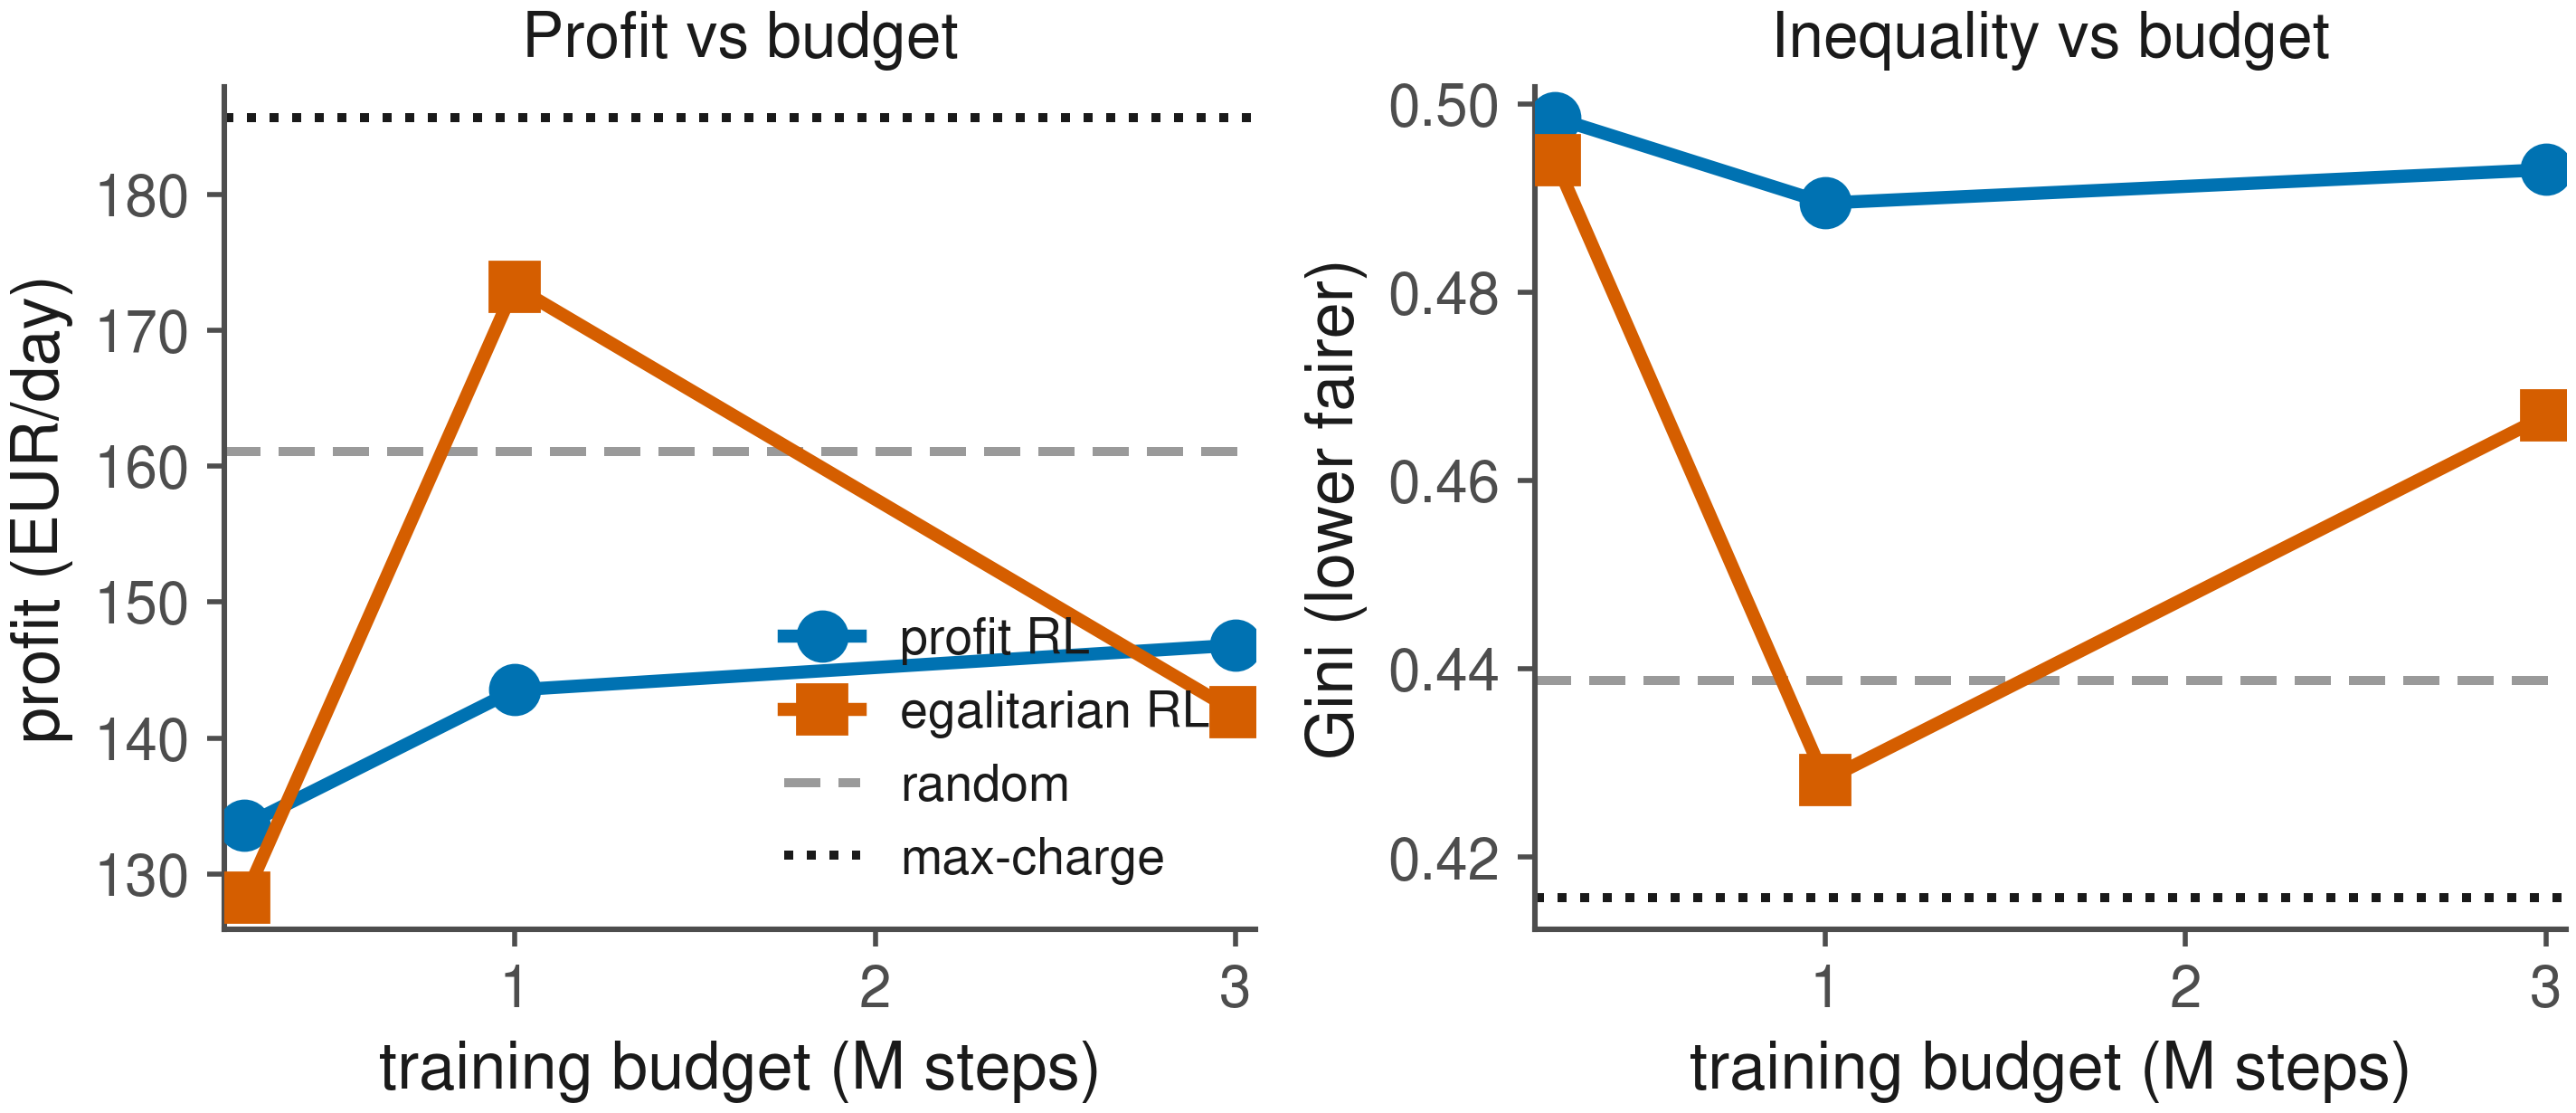
\includegraphics[width=\linewidth]{figures/learning_curve.png}
\caption{Learning curve diagnostic. Profit and Gini against training budget for the
profit and egalitarian configurations, with the random and max charge baselines as
horizontal lines. The learned policies are undertrained at the committed budget. The
egalitarian policy clears the random baseline at one million timesteps but is not yet
stable.}
\label{figcurve}
\end{figure}

\bibliographystyle{aaai}
\begin{thebibliography}{99}

\bibitem[Atkinson(1970)]{atkinson1970} Atkinson, A. B. 1970. On the Measurement of
Inequality. \textit{Journal of Economic Theory}, 2(3): 244--263.

\bibitem[Banerjee et al.(2022)]{banerjee2022} Banerjee, S.; Gkatzelis, V.; Gorokh, A.;
and Jin, B. 2022. Online Nash Social Welfare Maximization with Predictions. In
\textit{Proc. ACM-SIAM Symposium on Discrete Algorithms (SODA)}.

\bibitem[Barman, Khan, and Maiti(2022)]{barman2022} Barman, S.; Khan, A.; and Maiti,
A. 2022. Universal and Tight Online Algorithms for Generalized-Mean Welfare. In
\textit{Proc. AAAI Conference on Artificial Intelligence}.

\bibitem[Bednar and Reames(2020)]{bednar2020} Bednar, D. J.; and Reames, T. G. 2020.
Recognition of and Response to Energy Poverty in the United States. \textit{Nature
Energy}, 5: 432--439.

\bibitem[Borenstein(2012)]{borenstein2012} Borenstein, S. 2012. The Redistributional
Impact of Nonlinear Electricity Pricing. \textit{American Economic Journal, Economic
Policy}, 4(3): 56--90.

\bibitem[Burger et al.(2020)]{burger2020} Burger, S. P.; Knittel, C. R.;
Perez-Arriaga, I. J.; Schneider, I.; and Vom Scheidt, F. 2020. The Efficiency and
Distributional Effects of Alternative Residential Electricity Rate Designs.
\textit{The Energy Journal}, 41(1).

\bibitem[Caulfield et al.(2022)]{caulfield2022} Caulfield, B.; Furszyfer, D.;
Stefaniec, A.; and Foley, A. 2022. Measuring the Equity Impacts of Government
Subsidies for Electric Vehicles. \textit{Energy}, 248.

\bibitem[Drehobl, Ross, and Ayala(2020)]{drehobl2020} Drehobl, A.; Ross, L.; and
Ayala, R. 2020. How High Are Household Energy Burdens? Technical report, American
Council for an Energy-Efficient Economy (ACEEE).

\bibitem[Fan et al.(2023)]{fan2023} Fan, Z.; Peng, N.; Tian, M.; and Fain, B. 2023.
Welfare and Fairness in Multi-Objective Reinforcement Learning. In \textit{Proc.
International Conference on Autonomous Agents and Multiagent Systems (AAMAS)}.

\bibitem[Faruqui, Hledik, and Palmer(2011)]{faruqui2011} Faruqui, A.; Hledik, R.; and
Palmer, J. 2011. Time-Varying and Dynamic Rate Design. Technical report, Regulatory
Assistance Project and The Brattle Group.

\bibitem[Hassanzadeh et al.(2023)]{hassanzadeh2023} Hassanzadeh, P.; Kreacic, E.;
Zeng, S.; Xiao, Y.; and Ganesh, S. 2023. Sequential Fair Resource Allocation under a
Markov Decision Process Framework. In \textit{Proc. ACM International Conference on AI
in Finance (ICAIF)}.

\bibitem[Hsu and Fingerman(2021)]{hsu2021} Hsu, C.-W.; and Fingerman, K. 2021.
Public Electric Vehicle Charger Access Disparities across Race and Income in
California. \textit{Transport Policy}, 100: 59--67.

\bibitem[Jenkins et al.(2016)]{jenkins2016} Jenkins, K.; McCauley, D.; Heffron, R.;
Stephan, H.; and Rehner, R. 2016. Energy Justice, A Conceptual Review. \textit{Energy
Research and Social Science}, 11: 174--182.

\bibitem[Ju, Ghosh, and Shroff(2024)]{ju2024} Ju, P.; Ghosh, A.; and Shroff, N. B.
2024. Achieving Fairness in Multi-Agent Markov Decision Processes Using Reinforcement
Learning. In \textit{Proc. International Conference on Learning Representations (ICLR)}.

\bibitem[Khan, Tang, and Zhou(2022)]{khan2022} Khan, H. A. U.; Price, S.; Avraam, C.;
and Dvorkin, Y. 2022. Inequitable Access to EV Charging Infrastructure.
\textit{The Electricity Journal}, 35(3).

\bibitem[Lee, Li, and Low(2019)]{lee2019acndata} Lee, Z. J.; Li, T.; and Low, S. H.
2019. ACN-Data, Analysis and Applications of an Open EV Charging Dataset. In
\textit{Proc. ACM International Conference on Future Energy Systems (e-Energy)}.

\bibitem[Liu and Hajiesmaili(2025)]{liu2025} Liu, Q.; and Hajiesmaili, M. 2025.
Online Fair Allocation of Reusable Resources. In \textit{Proc. ACM on Measurement and
Analysis of Computing Systems (SIGMETRICS)}.

\bibitem[Mandal and Gan(2023)]{mandal2023} Mandal, D.; and Gan, J. 2023. Socially Fair
Reinforcement Learning. arXiv:2208.12584.

\bibitem[Mo and Walrand(2000)]{mo2000} Mo, J.; and Walrand, J. 2000. Fair End-to-End
Window-Based Congestion Control. \textit{IEEE/ACM Transactions on Networking}, 8(5):
556--567.

\bibitem[Moulin(2003)]{moulin2003} Moulin, H. 2003. \textit{Fair Division and
Collective Welfare}. MIT Press.

\bibitem[Mutti et al.(2022)]{mutti2022} Mutti, M.; De Santi, R.; De Bartolomeis, P.;
and Restelli, M. 2022. Challenging Common Assumptions in Convex Reinforcement
Learning. In \textit{Advances in Neural Information Processing Systems (NeurIPS)}.

\bibitem[Ng, Harada, and Russell(1999)]{ng1999} Ng, A. Y.; Harada, D.; and Russell,
S. 1999. Policy Invariance under Reward Transformations, Theory and Application to
Reward Shaping. In \textit{Proc. International Conference on Machine Learning (ICML)}.

\bibitem[Ponse et al.(2025)]{ponse2025} Ponse, K.; Kleuker, J. F.; Plaat, A.; and
Moerland, T. 2025. Chargax, A JAX-Accelerated EV Charging Simulator.
arXiv:2507.01522.

\bibitem[Rawls(1971)]{rawls1971} Rawls, J. 1971. \textit{A Theory of Justice}.
Harvard University Press.

\bibitem[Schulman et al.(2017)]{schulman2017} Schulman, J.; Wolski, F.; Dhariwal, P.;
Radford, A.; and Klimov, O. 2017. Proximal Policy Optimization Algorithms.
arXiv:1707.06347.

\bibitem[Sen(1999)]{sen1999} Sen, A. 1999. \textit{Development as Freedom}. Oxford
University Press.

\bibitem[Siddique, Weng, and Zimmer(2020)]{siddique2020} Siddique, U.; Weng, P.; and
Zimmer, M. 2020. Learning Fair Policies in Multi-Objective Deep Reinforcement
Learning with Average and Discounted Rewards. In \textit{Proc. International
Conference on Machine Learning (ICML)}.

\bibitem[Sinclair et al.(2022)]{sinclair2022} Sinclair, S. R.; Jain, G.; Banerjee,
S.; and Yu, C. L. 2022. Sequential Fair Allocation, Achieving the Optimal Envy
Efficiency Tradeoff Curve. \textit{Operations Research}.

\bibitem[Sovacool and Dworkin(2016)]{sovacool2016} Sovacool, B. K.; and Dworkin, M.
H. 2016. \textit{Global Energy Justice, Problems, Principles, and Practices}.
Cambridge University Press.

\bibitem[Zahavy et al.(2021)]{zahavy2021} Zahavy, T.; O'Donoghue, B.; Desjardins, G.;
and Singh, S. 2021. Reward Is Enough for Convex Markov Decision Processes. In
\textit{Advances in Neural Information Processing Systems (NeurIPS)}.

\end{thebibliography}

\end{document}
